\fancychapter{Indoor positioning}
\label{cap:indoor}

This chapter gives an overview of the state of the art of indoor positioning solutions.Section \ref{sec:techniques} starts by introducing the most common techniques used for location calculation, while Section ~\ref{sec:indoortech} overviews the existing indoor compatible technologies. Section ~\ref{sec:related} analyses the systems that had the most relevance in the field alongside existing \ac{BLE}-related systems. In Section \ref{sec:description} an overview of the existing formats for describing locations is given and finally, Section ~\ref{sec:critical} presents a critical overview of all the technologies and system previously presented in the chapter.

\section{Location calculation techniques} 
\label{sec:techniques} 
 
 
This section's focus is on the available means of obtaining distance measurements from a mobile target to a beacon. Figure \ref{fig:BeSP} displays a representation of the beacon-smartphone interaction. Whenever a location calculation is requested, the collection of data from nearby reference points is mandatory. In indoor location systems, these reference points are provided by beacons deployed in the location environment. The type of information collected, that is afterwards translated into distance, can be of several different types. The following section will target the different means of obtaining distances, as well as how to calculate a location from them.  

\begin{figure}[H] 
\centering 
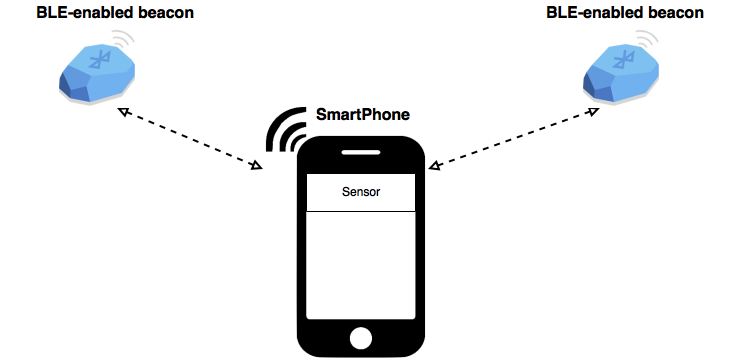
\includegraphics[width=0.65\linewidth]{2.Chapter/Beacon+SP.png} 
\caption[Beacon and Smartphone interaction]{Beacon and Smartphone interaction} 
\label{fig:BeSP} 
\end{figure} 

\subsection{Proximity Detection} 
\label{subsec:prox} 
 
 
Proximity detection is one of the simplest position techniques to implement since its objective isn't to provide a precise position of the target but a symbolic relative location information\cite{reviewtechniques}. The target's position is obtained through the \ac{CoO} method which relies on a grid of antennas/beacon with a well-known position. When applying this method, if only one beacon is detected by the mobile target then the position provided is equal to the position of the beacon. If more than one beacons are detected by the target, it considers that its position is equal to the position of beacon with the strongest associated signal. In order to apply room-based accuracy, the minimum requirement would be to place a beacon in each existent room. This method can be applied with a better accuracy in mind and doing so, it depends only on the deployed beacon density. This technique is often implemented in systems running \ac{IR} , \ac{RFID} and Bluetooth. 
 
 

\subsection{Triangulation} 
\label{subsec:tri} 
 

 
The Triangulation techniques make use of the geometric properties of triangles to determine the location of a mobile target. It can be of two types: lateration, which estimates a target's position by measuring its distance to multiple reference points, and angulation, which obtains the target's position by computing angles relative to multiple reference points. The metrics used for location calculation with either of the types, will now be presented. 



\subsubsection{Time of Arrival (ToA) } 
\label{subsubsec:toa} 
 
 
\ac{ToA}-based systems rely on accurate clock synchronisation and signal message sent from a mobile target to several receiving beacons \cite{locationtechniques}. The distance that is to be used in the calculation of the target's position is proportional to the propagation time. The message sent from the mobile target is timestamped with its departure time allowing for the receiving beacons to obtain their distance to the target through the transmission time and the associated signal propagation speed. 
One of the consequences of requiring precise knowledge of transmission start times is that every single device, beacon and mobile target, need to be accurately synchronised with a precise time source which causes this technique to be the most accurate one in indoor environments since it's capable of filtering multi-path effects. On the other hand, the disadvantages of using this technique is the synchronisation requirements and the additional information that needs to be contained in the sent messages, i.e. timestamps.  
 
 
 
 
\subsubsection{Time Difference of Arrival (TDoA) } 
\label{subsubsec:tdoa} 
 
 
\ac{TDoA} systems attempt to determine the relative position of a mobile target by examining the differences in time at which the signal arrives at multiple beacons\cite{TDoA}. This technique doesn't require clock synchronisation with the sender as there is no need for timestamps to obtain its location, making this requirement only present on the receivers. The location is obtained from a transmission with unknown starting time that is received in multiple synchronised receivers which produces multiple \ac{TDoA} measurements. Each difference in arrival times produces a \ac{TDoA} and consequently a hyperbolic curve on which the target is located. Each intersection of multiple hyperbolic curves represents a possible location of the target, requiring two or more measurements in order to obtain the location on a two dimensional plane. 
 
 
 
 
\subsubsection{Roundtrip Time of Flight (RToF)} 
\label{subsubsec:rtfo} 
 
 
This technique obtains distances by measuring the time-of-flight of the signal pulse traveling from the transmitter to the receiver ( measuring unit) and back\cite{rtfo}. This solution solves some of the synchronisation issues presented by \ac{ToA} since one of the two nodes records the transmission and arrival times, with the conversion from time to distance being equal to the one applied with \ac{ToA}. The mechanism of obtaining a time reading is similar to that of a radar, i.e. a signal is sent to the receiving node which replies back to the transmitter. When the response signal is received the roundtrip time is obtained. One issue presented by using this technique is the incapability of knowing the time delay on the receiver between receiving the first signal and sending the response. This unknown delay can be ignored in medium to long-ranged systems, if its value is relatively small when compared to the transmission time. In short-ranged system this situation can't be applied and therefore this technique isn't suited to be applied. 
 
 
 
 
\subsubsection{ \ac{RSSI}} 
\label{subsubsec:rssi} 
 
 
Received Signal Strength Information (RSSI) is a non-linear signal strength indicator based on signal attenuation that is only usable with radio signals. The conversion of this value to distance is often achieved through estimates of signal path loss due to propagation, although this approach doesn't hold in scenarios where severe multipath effects and shadowing are present. 
 
 
A technique that is often used with \ac{RSSI} is the fingerprint method which is the process of computing the location of a user by matching its location-dependent signal characteristics to an existing fingerprint database. This method doesn't require any additional hardware on the mobile device or the beacons as well as no time synchronisation. This process is divided in two stages: an offline and an online phase. In the offline stage, also called calibration phase, the maps for the fingerprint are set up either empirically in measurement operations or computed analytically through a signal propagation model. For the first option, multiple positions are defined on the map. On each of this positions a mobile user captures the signal strengths received from each of the existent beacons. An example of this method's data collection setup can be seen on Figure \ref{fig:fp}. With the fingerprint concluded, begins the online phase, where mobile users are already capable of being tracked. In order to obtain a user's position, it must measure the existent signal properties, which are then compared with the fingerprint database so that a close as possible match can be found. Position matching can be achieved through pattern recognition techniques such as K-nearest-neighbours (KNN), support vector machines (SVM), among others. 
This approach has the drawbacks of being labour intensive and time consuming on the offline phase and the difficulty to maintain and update the fingerprint database in order to be in accordance with the current environment. The second drawback is caused by \ac{RSSI}'s sensibility to changes in the environment such as dynamic factors (people and doors), diffraction and reflection.  
 
\begin{figure}[H] 
\centering 
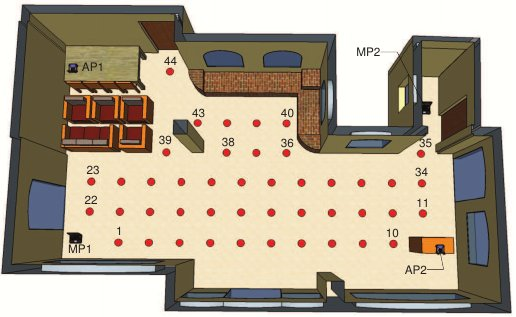
\includegraphics[width=0.5\linewidth]{2.Chapter/fp.jpg} 
\caption[Fingerprint example with data collection positions (Ref \cite{fingerprint}) ]{ Fingerprint example with data collection positions (Ref \cite{fingerprint}) } 
\label{fig:fp} 
\end{figure} 
 
 
\subsubsection{Angle of Arrival (AoA) } 
\label{subsubsec:aoa} 
 
 
The \ac{AoA} technique finds the location of the target by intersecting several pairs of angle direction lines. Each of these lines is part of the circular radius around a beacon which leads to the mobile target. This technique requires only two beacons for two dimensional and three for three dimensional position estimation, with any extra beacon leading to an increase in accuracy while not requiring any time synchronisation\cite{anglearrival}.  
This technique has two drawbacks: Increased implementation cost, since antennas capable of measuring angles are costly; Rapid accuracy degradation, i.e. the accuracy is heavily affected by the distance between user and beacon. This technique is capable of sub-meter accuracy although these types of systems are often limited by shadowing, multi-path reflections arriving from misleading directions or by the directivity of the measuring aperture.  
One example which attempted to tackle \ac{AoA}'s drawbacks was ArrayTrack \cite{arraytrack} which presented a multipath suppression algorithm capable of removing reflection paths, performance improvements in low density scenarios and parallel processing allowing for faster location estimations. This system was capable of achieving a median accuracy of 23 cm while utilising custom made access points with 16 antennas. Although successful, the hardware complexity remained an issue making this system impractical. 
 
 
\subsection{Dead Reckoning} 
\label{subsec:dr} 
 
 
\ac{DR} is the process of estimating the target's current position through the last determined position incremented by known or estimated speeds over elapsed time. This technique has the advantage of providing autonomous positioning capacities. \ac{DR} biggest drawback is that the inaccuracy of the process is cumulative, once the deviation in the position estimation grows with time. This issue can be aggravated by disruptive motion such as sidestepping, back-stepping or sharp turns which produce scaling errors leading to bigger accuracy errors. Due to \ac{DR}'s issues it's often accompanied by another technology in order to correct the inertial drift. A common practice is the usage of GPS, which doesn't function in indoor environments, leading to the implementation of many different combinations, in an attempt to tackle this issue. Fischer et al. \cite{dr1} made use of Ultrasound beacons as landmarks to provide better accuracy and less heading errors. In their work they stated the existence of two types of errors: heading errors, which are relative to the direction in which the user is heading, and distance errors. The work was targeted for rescue team first responders and required the users to drop ultrasonic beacons as they advanced through the building. 
\section{Indoor location support technologies}  
\label{sec:indoortech}  
  
  
When looking at the state of indoor positioning systems, it's clear that there isn't one technology that is better than all of the others. Therefore, it's important to look at each of the possible technologies individually and assess its benefits and drawbacks as well as their performance\cite{survey1}.  
  
  
In this chapter, many existent indoor positioning technologies are analysed. The most pertinent ones, \acf{RFID}, Commodity wireless technologies, Infrared, Ultra-wide band and Bluetooth low energy, are explained in a more detailed manner, while the less utilised technologies are described in Subsection \ref{subsec:others}. For each of the present technologies a description is provided about their nature, tags and pros and cons, all of which is complemented with at least one existent system that makes use of the specific technology being described.   
  
  
The information provided on each technology was gathered from a set of surveys on indoor location \cite{surveythesis,survey2,survey1}, as well as the information present on the mentioned systems associated to each.  
  
  
\subsection{RFID}  
\label{subsec:rfid}  
  
  
\ac{RFID} is a technology for storing and retrieving data through electromagnetic transmission to an RF compatible integrated circuit. A \ac{RFID} system is composed by three components: readers, tags and the communication between both. The reader is capable of reading the data that is being emitted from \ac{RFID} tags via radio waves and the data usually consists of the tag's unique identification number which can be related to the tag's available position information in order to obtain the user's position. This communication is achieved by having a well-defined radio frequency and protocol which allows for reading and transmitting data. The \ac{RFID} tags can be of two types: active or passive.  
  
  
Active tags are small transceivers equipped with an internal battery, which makes them heavier and more costly while allowing for longer detection ranges when compared to their counterparts \cite{surveythesis}. These tags are suited for identification of important units moving through rough processes or positioning in system where location estimation is often carried out through fingerprinting on \ac{RSSI}.  
Passive tags are operated without the need of a battery since they are capable of receiving enough energy in the form of radio frequency waves from nearby \ac{RFID} scanners in order to transmit back the answers. These tags are used to replace the barcode technology since they are much lighter, smaller and less expensive than the active tags which allows for a relative inexpensive installation and low maintenance caused by not having batteries. One of its drawbacks is that their range is very limited, circa 2 meters, which demands for higher density of tag deployment.  
  
  
\ac{RFID}'s biggest advantages are the non required \ac{LOS} characteristics, their capability of working at high speeds and their relative low cost\cite{survey2}. The non required \ac{LOS} characteristics comes from its radio frequency nature. Radio frequency signals are composed of electromagnetic waves and as such are capable of passing through obstacles at the cost of signal strength. As such this technology is often used for tracking objects in automobile assembly industry or warehouse management and tracking of people or animals.  
One of its most relevant projects is the SpotON \cite{spoton}, a tagging technology for three dimensional location sensing based on radio signal strength analysis. The tags used are custom devices that operate either standalone or as a plug in card enabling larger devices to take advantage of location-sensing technology. They are low power, small and capable of being accurate while having the computing capacity for relevant tasks such as caching, authentication, among others. SpotON tags utilise the received \ac{RSSI} as a metric for obtaining inter-tag distance.  
  
  
Another important project using \ac{RFID} is LANDMARC\cite{landmarc} which utilises active tags to produce a location sensing system for locating objects inside buildings. Its objective was to demonstrate that active tags can in fact be viable and cost-efficient for indoor location sensing. One of the problems found was that the hardware wasn't capable of providing \acf{RSSI} readings( a value used to evaluate the strength of a radio signal), as such the used readers scan through eight discrete power levels in order to estimate the \ac{RSSI}.   
  
  
\subsection{Commodity wireless technologies}  
\label{subsec:wifi}  
  
  
Commodity wireless technologies can be used to estimate the location of a mobile user that resides inside the network. Nowadays Wi-Fi positioning systems have become the most widespread approach for indoor location systems since \ac{WLAN} access points are readily available in many indoor environments and any Wi-Fi compatible device (smartphones, laptops, tablets) can be located without the need of installing extra software or manipulating the hardware. Its popularity is also due to its range of 100 to 50 meters and since \ac{LOS} isn't required. One issue of \ac{WLAN} signals is that they suffer attenuation from static environment such as walls and movement of furniture and doors. In these kind of systems position computation is obtained through TOA, AOA, RSS, and CSI, which are properly analysed in Section \ref{sec:techniques}, with multiple projects for each one of the existing methods. The most widely used is the \ac{RSSI}, which suffers from severe multipath effects leading to propagation model failures and as such inaccuracy in distance measurement. With these problems in mind a technique called RSSI-based fingerprinting is often used in order to improve performance.  
Most recently an alternative to RSSI has been researched called \ac{CSI}. \ac{CSI} is widely available on commercial products and it represents the channel conditions over individual OFDM subcarriers across the \ac{PHY} layer. One of the improvements is that instead of obtaining one \ac{RSSI} value per packet, multiple \ac{CSI} values can be obtained from multiple subcarriers at a time. FILA \cite{fila} was a project that attempted to use \ac{CSI} for locating targets in complicated indoor environments where RSSI wasn't reliable due to multipath. This system is capable of extracting the \ac{LOS} path for distance calculation through time-domain multipath mitigation and frequency-domain fading compensation and with a simple trilateration calculation they were able to achieve a much better performance than with \ac{RSSI} for these kind of scenarios. The performance comparison showing the differences in temporal stability between \ac{RSSI} and \ac{CSI} can be seen on Figure \ref{fig:fila}.  
  
  
\begin{figure}[H]  
\centering  
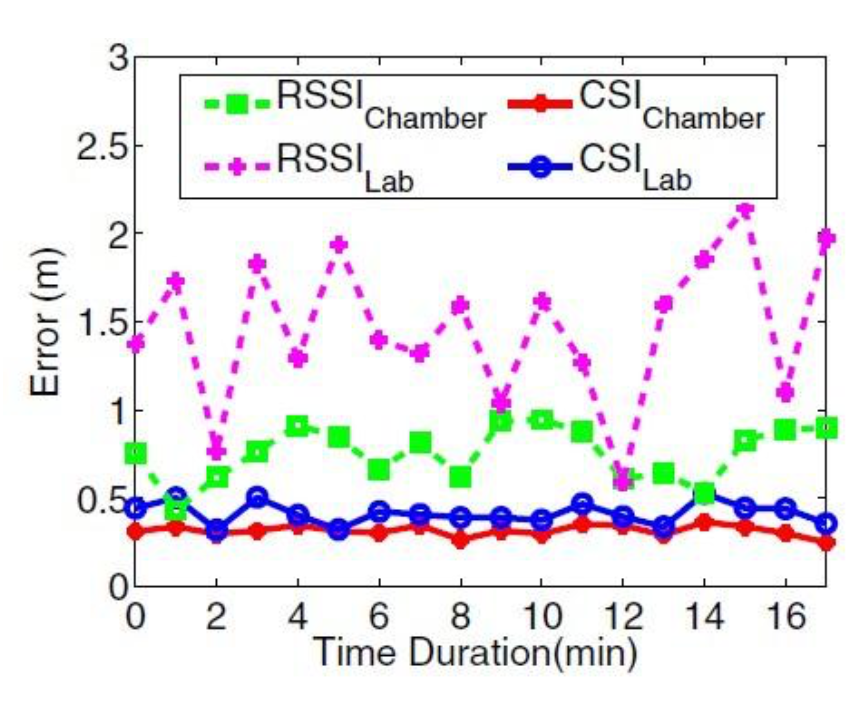
\includegraphics[width=0.5\linewidth]{2.Chapter/fila-comparison.png}  
\caption[Comparison of temporal stability (Ref \cite{fila}) ]{Comparison of temporal stability (Ref \cite{fila})}  
\label{fig:fila}  
\end{figure}  
  
  
  
  
\subsection{Bluetooth low energy}  
\label{subsec:ble-tech}  
  
  
Bluetooth low energy was introduced as an improvement to the already existent Bluetooth, aimed at Internet of Things (IoT). Its most relevant improvements from the classic Bluetooth were the reduced power consumption, lower complexity and lower power consumption. \ac{BLE} operates in the same frequency range as the classic Bluetooth, allowing them to make use of the same antenna, and as Wi-Fi. This technology is known for its short-range, overall low power consumption and low-cost transceiver chips.  
\ac{BLE}'s initial target was localised advertising and "near-me" applications, due to its proximity sensing capacity. Nevertheless, its viability as an indoor location technology has been studied, showing that it can be used alongside fingerprinting or with proximity detection. Both techniques make use of \ac{RSSI}, which in the case of \ac{BLE} is not a reliable measure. This condition is caused by the sharing of the same frequency band as Wi-Fi, leading to possible signal interference that causes signal fluctuation. In Section \ref{subsec:ble}, examples of \ac{BLE} systems are provided.  
  
  
\subsection{Infrared}  
\label{subsec:ir}  
  
  
\ac{IR} systems are mostly used for tracking objects or people. \ac{IR} wavelengths are invisible to the human eye under most circumstances, making this technology less intrusive than those which are visible. This technology is widely available in various common devices such as mobile phones, PDA's and TV's and requires \ac{LOS} communication between receiver and transmitter, preferably without interference from strong light sources. One of the most relevant systems based on \ac{IR} is the Active Badge system which is described in Section \ref{sec:related}. There are three methods of exploiting infrared signals: through active beacons, infrared imaging or artificial light sources.  
  
The active beacon's approach is the one employed by the active badge system and it involves placing fixed \ac{IR} beacons on known positions. The density of deployment of beacons has a direct impact on the system's accuracy. If a system was required to achieve room-based accuracy, i.e. being able to tell in which room a user is located, a beacon per room would be sufficient.   
  
Infrared imaging, also known as passive \ac{IR} systems, makes use of sensors operating in the \ac{IR} spectrum which are capable of obtaining a complete image of the surrounding from thermal emissions. This approach doesn’t require the deployment of any extra hardware or tag for determining the temperature of objects or people but it does get compromised in the presence of strong radiation from the sun. Some known equipments that use this approach are thermal cameras, infrared sensors for motion detection or thermocouples used to measure temperature contact free.   
  
\ac{IR} systems based on artificial light sources are a good alternative to the ones that operate on the visible spectrum. A very well known example is the Microsoft Kinect system which uses continuously‐projected infrared structured light to capture 3D scene information with an infrared camera. This system is capable of tracking a person's movement up to 3.5 meters with a precision of a few centimeters.   
  
\subsection{Ultra-Wideband}  
\label{subsec:uwb}  
  
  
\ac{UWB} is a radio technology aimed at short-range high-bandwidth communication. Its best characteristics are the capacity of being resistant to multipath and to some degree being capable of penetrating building materials, such as concrete and wood, with low power consumption. Both these factors allow \ac{UWB} to achieve high positioning accuracy while the latter enables to address the range in non line-of-sight conditions and makes inter-room ranging possible. Being able to penetrate building material creates precision issues due to the increase in data complexity, making data interpretation one of the biggest challenges to be faced. The usual structure of a \ac{UWB} system has a stimulus radio wave generator and receivers which capture the propagated and scattered waves and it has four types of methods for position calculation.  
The first one, passive \ac{UWB}, attempts to track objects or people through signal reflection. This method doesn't require any sort of tag to be carried by the user or attached to the object and requires only at least on emitter and a few listeners to obtain a location. Since the locations of the antennas are known and it is possible to estimate the distance from user to listener through \ac{ToA} or \ac{TDoA} multilateration, the user's location can be computed.  
The remaining methods are Direct Ranging and Fingerprinting. The first one simply requires the users to wear active tags and uses different measures based on time to compute distances which are then worked by lateration techniques in order to produce the user's location. The second one works like a regular fingerprinting method except that it employs Channel Impulse Response (CIR) instead of \ac{RSSI}. This kind of fingerprinting has the possibility of being more accurate while being usable in non \ac{LOS} scenarios. On the downside it requires time synchronisation.  
One commercial example of this technology is Ubisense \cite{ubisense}, a system capable of tracking active tags equipped with batteries which have a conventional RF transceiver and a \ac{UWB} transmitter. The system requires a setup deployment of a network of Ubisensors, with fixed positions throughout the area to be covered and networked using Ethernet. Each sensor has a RF transceiver and  phased array of \ac{UWB} receivers. These sensors use a combination of \ac{TDoA} and \ac{AoA} techniques to determine the tags location, achieving an accuracy of 15 cm in a typical open environment. The system's setup can be visualised on Figure \ref{fig:ubisense}.  
  
  
  
  
\begin{figure}[H]  
\centering  
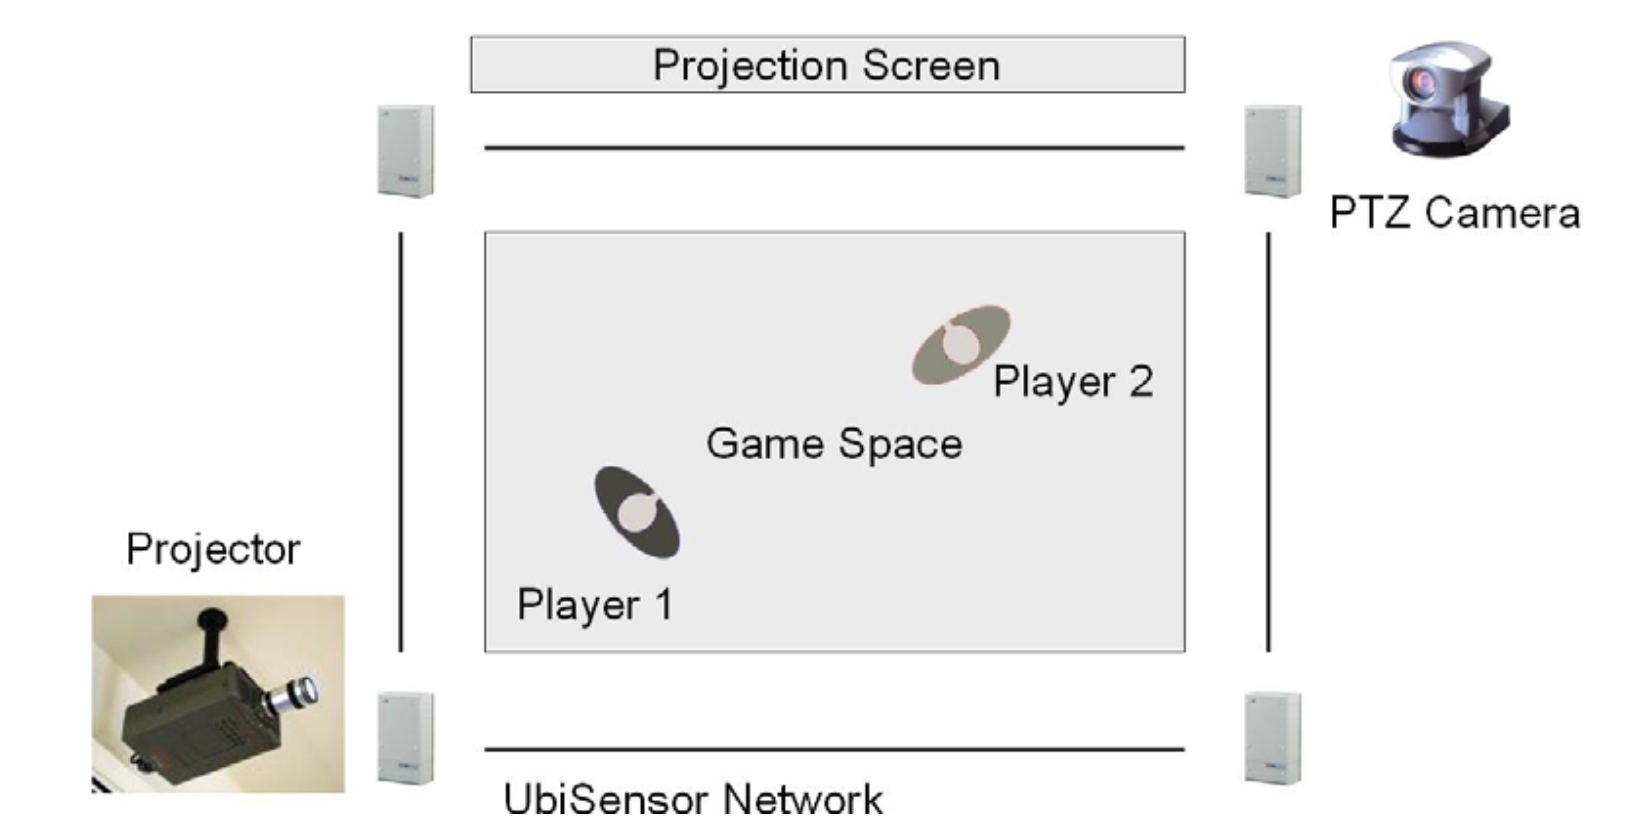
\includegraphics[width=0.7\linewidth]{2.Chapter/ubisense.png}  
\caption[Ubisense's system setup (Ref \cite{ubisense}) ]{Ubisense's system setup (Ref \cite{ubisense})}  
\label{fig:ubisense}  
\end{figure}  
  
  
  
  
\subsection{Other systems}  
\label{subsec:others}  
  
  
\begin{description}  
  
  
\item [Optical]  Indoor positioning systems are systems that use a camera as their only or main input for position estimation. In recent years these types of systems have found an increase in success due to the improvements and size reduction of the sensors, the improvements in computational capacities and the continuous development of image processing algorithms. Optical systems can be described as a moving sensor, for example a smartphone camera, and often times a set of static sensors which detect movement and which employ \ac{AoA} techniques to estimate distances. There are many different types of optical systems, one of them makes use of 3D building models. This approach removes the need for local infrastructure deployment in the building to be monitored since the usually required reference nodes are replaced by a digital reference point. As such they are highly scalable with small increases in cost.  
In general optical systems are capable of achieving high accuracy but they are vulnerable to light conditions, require \ac{LOS} propagations and are more computationally expensive than other types of systems.  
  
  
  
  
\item [\ac{FM} radio]  Is a broadcasting technology that has been incorporated for a long time on smartphones with the intent of listening to music or to the news. This technology was originally reserved for frequency modulation to convey information over a carrier wave by varying its frequency but nowadays it just refers to any radio wave in the frequency band 88-108 MHz. This analogue radio signal has amazing advantages for urban/indoor location system such as the ability to be received indoor and outdoor, it has a dense coverage in urban areas, available without installing additional transmitters, low-cost and low-power hardware with simple technology, high received signal power and there are a large number of transmitters which provides good geometry for locating. One crucial part when using \ac{FM} is that it doesn't carry any timing information which is critical in range calculation and the fact that as other radio frequency technologies, it suffers from  multipath effects and non-\ac{LOS} signals. An example of FM system was created by  et al. \cite{fm} which implemented an \ac{RSSI} fingerprint-based system using FM radios in an office environment. The system's test bed obtained 17 FM channels at each point of the fingerprint and it was capable of achieving a mean accuracy of 3 meters.  
  
  
  
  
\item [ZigBee]  Is an emerging wireless technology standard which provides solution for short and medium range communications and its specially designed for applications which demand low-power consumption and don't require large data throughput. This technology's signal range coverage can go up to 100 meters in open space, while achieving 20 to 30 meters in indoor environments. Most ZigBee-based system employ \ac{RSSI} for distance calculation and one of its most relevant disadvantage is its vulnerability to interference from a wide range of signal types using the same frequency which can disrupt radio communication. This is caused by ZigBee operating in the unlicensed ISM (industrial, scientific and medical reserved) bands. An example of a ZigBee-based system is the one created by Larrañaga et al. \cite{zigbee} which attempted to locate a mobile device in an indoor environment. Their system consisted of two phases:  
\begin{itemize} 
\item In the first phase, calibration, every ZigBee node communicated with the remaining. In this way, it was possible to work out the relationship between measured \ac{RSSI} values and geometric distances, allowing to map the environment. 
\item In the second phase, location, the mobile device communicated with the existing ZigBee nodes. This information, together with the one from the previous phase, was used to calculate the device's location. This system was capable of achieving an accuracy with an average error of 3 meters.    
\end{itemize} 
  
  
  
\item [Ultrasonic ]  Systems are employed in indoor positioning by making use of \ac{ToA} to locate targets\cite{survey3}. These kind of system make use of ultrasonic transceiver to emit and detect signals while recording times of departure and arrival of the signal. Since the signal medium traveling speed is known, it is possible to use the time difference to compute the distance between emitter and receiver.  One of the most famous projects that makes use of this technology is the cricket system which is described in Section \ref{sec:related}.  
  
  
\end{description}  
  
  
\subsection{Hybrid systems}  
\label{subsec:hybrid}  
   
Hybrid positioning systems combine several different positioning technologies to determine the location of a user or object. Hybrid systems make use of multiple technologies in an attempt to compensate for one's shortcomings through another's strengths. One example of an hybrid system is the solution presented by versus \cite{versus} which makes use of Wi-Fi, IR and RF to provide a system capable of displaying real-time locations of people or objects inside a building. By combining these three technologies their were capable of providing a system with different level of accuracy depending on the needs, room-level, bed-level (a fragment of a room) or chair-level (precise positioning).   
  
  
  
 
\section{Indoor location systems}  
\label{sec:related}  
  
  
\subsection{Active Badge}  
\label{subsec:badge}  
  
  
In 1992 the Active Badge system \cite{badge} was presented as an infrared solution capable of providing room-based position tracking. The system has been designed to make use of "active badge" beacons, which can be visualised in figure \ref{fig:badge} in the form of ID cards, a tag equipped with an \ac{IR} LED that emitted a unique code for approximately a tenth of a second every 15 seconds.  
  
  
\begin{figure}[H]  
\centering  
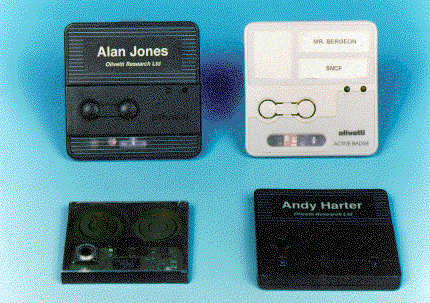
\includegraphics[width=0.5\linewidth]{2.Chapter/badges.png}  
\caption[Active badge's tags (Ref \cite{badgefig}) ]{Active badge's tags (Ref \cite{badgefig}) }  
\label{fig:badge}  
\end{figure}  
  
  
The decision to use \ac{IR} was caused by the small and cheap characteristics of the emitters and detectors\cite{badge2}. By being capable of operating within a 6 meter range, \ac{IR} signals aren’t capable of traveling through walls. The signal frequency has two major effects on the system: Firstly it impacts the tag's energy consumption, where a small frequency allows for long periods of work on a single battery; Secondly it impacts on user detection accuracy. For the used signal duration and frequency there is a chance of 1/150 for two signals to collide, which leads to a good probability that for a small number of beacons, all will be detected. One downside of such a small frequency signal is that the location of a badge can only be known, at best, with a 15 second granularity.  
  
The position of a user is obtained through the implementation of a network of sensors which act as receivers, continuously listening to badge transmissions. Upon collecting a transmission, the obtained information is sent to the master station. The master station is responsible for polling all the sensors on the network, storing sighted badges into a database where its associated time, position and ID are stored, data processing and data display. The accuracy of the system is room-based by making use of \ac{CoO} and the properties of \ac{IR}. A beacon in each room would make it so that each beacon is capable of detecting any badges in its room \cite{badge1}.  
  
  
\subsection{Active Bat}  
\label{subsec:bat}  
  
  
In 2001 the Active bat system \cite{bat}was introduced. It is a system capable of tracking various object, each tagged by attaching small wireless transmitters called bats. The system's architecture is composed of small devices named bats, which are to be carried by the objects or people to be tracked, a network of \acf{US} receiver units and several base stations\cite{bat1}. The receiver network and a deployed bat can be seen on figure \ref{fig:bat};  
  
  
\begin{figure}[H]  
\centering  
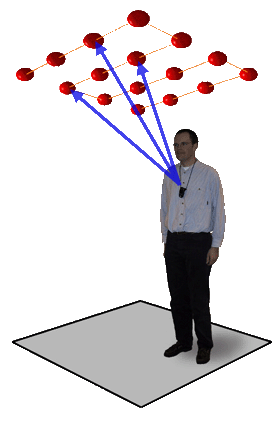
\includegraphics[width=0.5\linewidth]{2.Chapter/batarch.png}  
\caption[Active bat network and device(Ref \cite{batfig}) ]{Active bat network and device (Ref \cite{batfig}) }  
\label{fig:bat}  
\end{figure}  
  
  
A bat, which can be seen in figure \ref{fig:bat} being carried by the user, consisted of a radio transceiver, controlling logic and a ultrasonic transducer, each having an associated globally unique ID. A Base station periodically transmits a radio message containing a single unique ID, making it so that the ID's associated bat emits a short pulse of ultrasound. From this point on, the receivers monitor for the expected \ac{US} signal while recording the time spent waiting in order to obtain the signal's \ac{ToA}. With a known speed of sound in air, which can be estimated from the ambient temperature, the \ac{ToA} can be converted into bat-receiver distance.  
  
  
The mobile target's position can be obtained through multilateration in three dimensional space, for as long as three or more non-collinear receivers' distances are known. This method's accuracy is highly dependent on the distance measurement's accuracy. Distance measurement is affected by signal reflections on objects present in the environment, a problem that was correct by the use of a statistical outlier rejection algorithm. One other issue is the reverberations of the initial signal, which are required to die out before initiating another distance measurement in order to ensure that the incoming \ac{US} signals are from the correct bat. As such the measurement process is divided into time-slots, each being capable of locating one and only one bat.  
  
  
The latest version of the bat included a sensitive motion detector that allowed it to tell the base stations whether it was moving or stationary. Since the base station doesn't require to repeatedly determine the location of a stationary object, the system places these bats into a low-power sleep state which is only removed once the bat starts moving. This implementation allowed for extra power savings while freeing up location-update opportunities for other bats \cite{bat2}.  
  
  
\subsection{Radar}  
\label{subsec:radar}  
  
  
In 2001 the RADAR system was introduced as the first Wi-Fi signal-strength based indoor positioning system \cite{radar}. The system is Radio Frequency-based and its capable of locating and tracking users inside buildings. Radar makes use of signal-strength information obtained through a fingerprint method, presented in subsection \ref{subsubsec:rssi}, to triangulate the user's coordinates. The system's functions in two phases: the data collection phase, where the data is gathered in order to later construct and validate models for signal propagation, which are to be used in the real-time phase to infer user's location. In the offline phase, the type of data collected is the signal strength utilising the methodology already described for the fingerprint method.  
  
  
Radar's architecture involved a mobile device, base stations and a central station. The mobile device is solely responsible for sending signals to the base stations. During the process of developing the system, the device was a Windows-based mobile host capable of broadcasting packets. The base stations act as gateways, in a way that it listens for the user's signals and consequently forwards its information to the central station. The central station is in charge of storing the whole fingerprint information in the offline phase and calculating the user's location during the online phase.  
  
  
Data processing involved computing the mean, the standard deviation and the median of \ac{RSSI} for each of the used base stations (three in total) and each combination of x,y and direction. In addition, a building layout information was created which included room and base station's coordinates and the number of walls that obstructed the direct line between the base stations and each of the positions where data was collected. With all this information an accurate signal propagation model was built.  
  
  
The basic approach used to obtain a user's location was triangulation, which given a set of \ac{RSSI} measurements at each base station, the user's location is predicted to be the one that best matches the observed data. In addition to this basic strategy, two others approaches were analysed: empirical and signal propagation methods.   
  
  
For the first method many variations on the data were studied such as: The number of best matching values used ( K-nearest neighbours (KNN)). The results showed that the benefits of averaging between multiple neighbours isn't very relevant, even for small values of k. In general the empirical method was capable of estimating the user's location with high accuracy, obtaining a median error distance between 2 and 3 meters. Its main drawback being the required effort for building the data set for each physical area of interest. Another issue is the requirement to remake the data collection phase whenever a base stations is moved or there are heavy changes in the environment.  
  
  
The signal propagation model comes as an alternative to the empirical method for constructing the fingerprint. This method makes use of a propagation model for the signal to generate a set of theoretically-computed signal strength data, similar to the one physically collected. The performance of this method is correlated to how well the used model is capable of correctly describing the signal. This model provides a more reasonable way of obtaining data, since it doesn't require detailed and costly measurements. When compared to the empirical method, it was capable of achieving a mean error distance of 4.5 meters. Although it isn't as accurate, it can be considerate as a solution when analysing its benefits.  
  
  
\subsection{Cricket}  
\label{subsec:cricket}  
  
  
The Cricket system\cite{cricket} was developed by the Massachusetts Institute of Technology (MIT) in 2005 and managed to tackle some of the problems existent in the previously mentioned systems. The system makes use of nodes, small hardware platforms, consisting of a RF transceiver, a microcontroller and hardware capable of generating and receiving ultrasonic signals. There are two types of nodes: beacons, which are fixed reference points attached to the ceiling or walls of the building, and receivers, called listeners, which are attached to the objects that need to be tracked. Each beacon periodically transmits a \ac{RF} signal message containing beacon specific information, such as the beacon's unique ID, its coordinates and the physical space associated to the beacon. Whenever a \ac{RF} signal is transmitted, an ultrasonic pulse, which doesn't contain any data, is also emitted thus enabling listeners to measure their distance to the beacons by using the time difference of arrival times of the RF and ultrasonic signals. Each listener utilises the RF signal's beacon information alongside the obtain distances to beacons to compute their space position and orientation.   
  
  
When a beacon is deployed it doesn't know its exact position, only a human-readable string which describes its location. In order to compute the recently deployed beacon's position a listener is attached to a roaming device in order to collect distances from the beacons to itself. These distances are used to compute inter-beacon distances, which, when in high enough number, are capable of uniquely define how beacons are located in respect to each other. With this information it is then possible to obtain the beacon's coordinates.  
  
  
Cricket's architecture is completely decentralized, since it doesn't require a central node. The used nodes are responsible for communicating with the beacons and calculating its own location, while the beacons are responsible of finding their positions and transmitting their information to the listeners.  
  
  
The utilised method for computing distances doesn't require listeners to actively transmit messages which permits cricket to perform well independently to the number of users. This active-beacon passive-listener architecture makes it so that the position of the user isn't tracked by the system thus solving the user privacy that were present in the remaining projects.  
  
  
\begin{figure}[H]  
\centering  
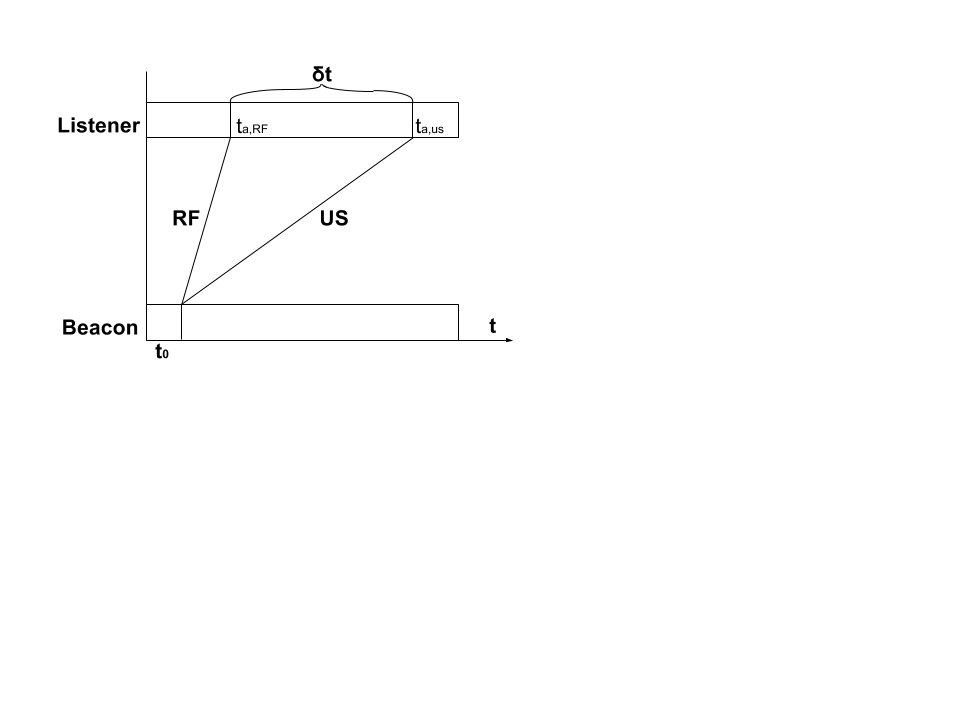
\includegraphics[width=0.5\linewidth]{2.Chapter/cricket-dist.png}  
\caption[Cricket's \ac{TDoA} representation]{Cricket's \ac{TDoA} representation}  
\label{fig:cricket-tdoa}  
\end{figure}  
  
  
Distance measurement is computed through \ac{TDoA} using both \ac{RF} and \ac{US} signals and it can be visualised in figure \ref{fig:cricket-tdoa}. Since the velocity of the \ac{RF} signal is much higher than that of the \ac{US} signal and when considering a direction, the \ac{US} signal lags behind when compared to the other. As such, whenever a listener receives a \ac{RF} signal, it measures the time it takes until the \ac{US} signal arrives, denominated $\delta{T}$. With knowledge of the speeds of sound and light, the distance between beacon and listener can be obtained from:  
  
  
\begin{equation}  
\delta t = \frac{d}{v_{US}} - \frac{d}{v_{RF}}  
\end{equation}  
  
  
This approach to distance computation is vulnerable to a certain amount of factors such as: Environmental factors since the velocity of sound depends on factors such as temperature, humidity and atmospheric pressure; Lack of \ac{LOS} since in these scenarios there is no \ac{LOS} between the beacon and the listeners, the \ac{US} signal may reach the listener after it has reflected on a surface. Reflection and refraction cause the signal to travel a longer distance than the direct path; Errors in detecting \ac{US} due to the threshold-based approach to detect the signal; \ac{TDoA} associated errors, which are associated to errors from time measurement and errors from detecting the \ac{RF} signal.  
  
  
In terms of performance, Cricket was capable of a distance measurement accuracy of 4-5 cm within a 80 degree cone from a given beacon, position accuracy of 10-12 cm and an orientation accuracy of 3º - 5º.  
  
  
\subsection{BLE systems}  
\label{subsec:ble}  
When looking at what's possible to achieve using the BLE technology there is the example of Apple's creation iBeacon \cite{ibeacon} which was presented in 2013 with the purpose of implementing proximity sensing systems. The devices are implemented as broadcasters, making it so that its objective is to send information to nearby compatible receivers. Some examples of application are to track customers or trigger location-based actions on devices such as push notifications or checking in on social media, with practical cases such as the usage of iBeacons by McDonalds to offer special offers to their customers in their fast-food stores. An indoor location system using this technology was presented by Jingjing Yang et al \cite{ibeacon1}, where these devices were used to indicate a patient of his whereabouts through the proximity sensing properties and this information was later transferred over to a server in order to give clients a variety of different services, from patient counting, to nearby department's information and offer indoor guidance to the nearest available bed.   
  
  
When utilising BLE for indoor location, the metric used to calculate distances is the RSSI. This metric within the context of Bluetooth brings to the surface several issues such as the fact that RSSI as a metric is very accurate only when the target is within a meter of the beacon, since the value decreases as the inverse of the square of the distance to the beacon. As such when developing solutions for indoor location that require systems with high accuracy capable of tracking moving objects, the usage of RSSI can't be utilised without further work. Faragher et al \cite{bleacc} tackled one of the techniques used to improve BLE system's accuracy, fingerprinting, by verifying the effects caused by the device deployment density within the required location. This experiment also puts into evidence one of the downsides of the Bluetooth technology, being that its scalability is low, besides requiring higher density in order to increase accuracy, due to their low range any need to increase coverage leads to increased costs.  
  
  
  
  
Zonith \cite{zonith} introduced a Bluetooth based location system with the objective of tracking the position of workers in dangerous environments. Any device registered in the zonith implemented network would be continuously tracked and accounted for in each of the system's functionalities such as, sounding an alarm whenever a lone worker doesn't move or respond within a time interval (Lone worker protection) or providing a quick a precise location of any worker that has requested for help. This system's installation requires planning of the best locations to place the beacons and number of beacons required, in order to be able to provide enough coverage and assure the system's required quality.  
  
 
\section{Location description formats} 
\label{sec:description} 
 
 
In order to better understand the existent various ways of describing locations it's better to look at existing solutions and the methods they employ. The most common method of describing location is through latitude and longitude, much like the \ac{GPS} does, with the biggest example that makes use of it being Google maps. Google maps, through its indoor maps platforms \cite{googlemaps} allows integration of indoor maps onto their google maps. Since Google Maps uses this type of location description, the indoor component of it follows the same routes. An indoor map on the platform is inserted into its original geographical location and in the case of having multiple floors, it is possible to navigate through them. This indoor component is of relatively small complexity, likely due to google's reduce investment onto indoor location system, leading to a small amount of indoor specific characteristics.  
 
 
Another method is to consider the indoor map as the location reference and utilise a cartesian coordinate system, x and y, to represent a location. Meridian, an indoor location system developed by HP \cite{meridian}, presents functionalities such as route making and push notifications through its beacons. The indoor map insertion is accomplished through Meridian's online platform. As such there isn't the outdoor component that google indoor maps has but it allows for utilising a (x,y) system relative to the building map. While no complex building description is allowed, it is still possible to indicate the position of specific elements such as restrooms or stores. 
 
 
Although Meridian already provides some extra level of detail in comparison with google indoor maps, there is another example that should be mentioned called OpenStreetMap. Although it started much like google, providing global data, due to its openness, many indoor projects surfaced such as OpenLevelUP \cite{openlevel}. This project makes use of OpenStreetMaps' current indoor tagging scheme \cite{opentagging}, which is intended to describe in the most complete and simple way a building. This makes available the number of floors, the type of elements (room, wall, corridor, etc) and its connectors, like doors and escalators or elevators, allowing to understand clearly the map that is being analysed. 
 
 
 
\section{Critical evaluation} 
\label{sec:critical} 
 

In this section we want to review all the technologies that have been presented in this chapter but this time comment and evaluate them with a modern day's vision. It is of relevance to understand which technologies present concepts that can still be easily usable in the present and whether or not they can be adapted to function with state-of-art smartphones. There are four core concepts that will be analysed: The level of difficulty in deploying the system; the accessibility of the system towards users, mainly focused on the compatibility with modern smartphones; the scalability of the systems; and finally the privacy of the systems. 
 
 
\subsection{Deployment of beacons and scalability} 
\label{subsec:dep} 
 
 
When deploying a system, there are factors that determine how troublesome it is. One factor is the cost of the beacons. Costly beacons can be an obstacle when the number of beacons required to be deployed increases. This number depends on the range and the precision demanded. 
A system's scalability depends on the possibility of increasing the infrastructure and covered area, as well as being capable of handling an increase in the number of users.  
Due to the high number of various technologies and correspondent systems, each one will be analysed separately. 
 
 
\begin{description} 
\item [\acf{RFID}]  The analysis of this technology can be achieved through one of its systems. A recent one was presented by Han Zou et al. \cite{rfid_sys} which makes use of RFID tags and sensors, a \ac{RFID} reader and a location server. The general procedure for calculating a location is:  
\begin{itemize} 
\item The tags emit their ID, which is caught by the sensors; 
\item The sensors make use of its external power supply to allow the creation of a continuous wireless connection with the reader. It's through this connection that any captured tag information is sent; 
\item the reader receives the data and forwards it to the server where the location is obtained. 
\end{itemize} 
This system introduces one of the issues of RFID which is the high cost of readers. 
In this type of architecture, where the objective is for tracking, the deployment of beacons is equivalent to deploying sensors and readers on the areas that are to be covered. As such, increasing the covered area ends up being a costly operation. Nevertheless, since tags are cheap and a user is required to carry just one, user scalability isn't an issue. 
 
 
When envisioning a \ac{RFID} system centralised on the users, the roles associated to the tags and sensors plus readers are exchanged. As such, in this scenario, the user scalability would be costly. This occurs since each user would be required to carry a reader. With the reference points being provided by \ac{RFID} tags, the covered area expansion becomes a cheap operation. 
 
 
\item[Commodity wireless technologies] In order to study these technologies, the radar system will be used. 
 
 
Radar's architecture defines the mobile user as the broadcaster for the whole of its process, be it offline and online phases of the fingerprint method as described in section\ref{sec:related}. Radar's deployment is dependant on a grid of access points and devices for each user. Nowadays both dependencies are often unnecessary since all mobile devices can use Wi-Fi and many indoor environments are already equipped with Wi-Fi access. Due to its wide availability, these system's deployment costs low when compared to other technologies.  
Despite the architecture, P. Bahl et al\cite{radar1} comment on its consequences, imagining that in a real situation, since the number of mobile users is vastly bigger than that of base stations, the inversion of the roles would be beneficial in order to decrease the complexity and the workload. 
Passing the broadcast role to the base stations while having the mobile users function as listeners, would make it so that for a certain floor the complexity would be constant, i.e. equal to the number of stations, instead of being unstable like the number of mobile users. This changes would increase the scalability in terms of users for this system. 
 
 
Wi-Fi systems often calculate a users location through either trilateration or fingerprint. In the case of fingerprint, the one used by Radar, the complications associated to the technique can reduce scalability. When compared to other techniques, this one has additional maintenance concerns, since it's not about changing a beacon or its location but about updating the areas fingerprint. When an update is required, the whole process must be redone, leading to high costs that are associated to the coverage of the system. 
  
 
 
\item[\acf{IR}] An example of a recent system based on this technology is the Epsilon project\cite{epsilon}, which makes use of Light-emitting Diode (LED) and light sensors.   
 
 
Epsilon makes use of LEDs and their capacity to both illuminate and communicate. Through the LED's ability to instantaneously change between on and off state, it is possible to carry digital data in the visible light carrier through Pulse Width Modulation (PWM). In this system each of the used LEDs was self-contained, i.e. it knew its own location, which was inserted into the data transmitted to the mobile user. The mobile user would capture the LED information through its light sensor, and consequently decode the received data from each of the available sources in order to make use of trilateration to obtain its position. 
 
 
Epsilon presents a solution which is easy to use in today's world due to the availability of LED lighting in indoor environments. Much like the systems that profit from Wi-Fi, this one is capable of profiting from the existing infrastructure for its deployment. The associated cost would then be associated to the adaptation of infrastructure to the one required by the system. For the mobile users, with the required sensors being available in most smartphones, the deployment isn't a problem. 
 
 
Epsilon's architecture was created with the intention of having a "plug-and-play" kind of system, made possible through the self-contained LEDs and location calculation made on the smartphone. These characteristics have an impact on the system's scalability. 
When presenting the system, the authors suggest a way to tackle this issue. Through the use of a back-end service for mapping the IDs of each LED to their location and by transferring the location calculation algorithm to it. This addition to the current architecture would boost the system's scalability since whenever an update or modification to the system's algorithm is required, interaction with every single device is required. 
 
 
 
 
\item[\acf{UWB}] This technology isn't practical for personal indoor location in today's world. The main reason is dependency on system specific hardware which invalidates the possibility of having a wide scale indoor location systems. 
 
 
When analysing recent \ac{UWB} systems, the most common ones are tracking only systems. These systems are found useful in construction environments, where tracking crane's position is of relevance \cite{uwb-ex1}. This position tracking is accomplished by setting up a network of \ac{UWB} sensors on the construction site and placing \ac{UWB} tags on the crane or parts of it, if the whole position and pose of the vehicle are of relevance, that is to be tracked. While the addition of new target implies only the deployment of new tags, the sensors high cost are the limiting factor on the technology's deployability and scalability.  
 
 
Despite the difficulty, Decawave \cite{uwb-ex2} attempted to introduce an indoor location solution. Decawave presents a \ac{UWB} transceiver in the form of a hardware module. The deployed beacons would be the traditional LED lights, with the addition of an \ac{UWB} transceiver, allowing them to communicate with the mobile user's device. Since this device would still be system-specific, the system's deployability and scalability are still reduced. 
 
 
\item [Optical] As described in section \ref{subsec:others}, optical systems are systems which are dependent on cameras, as means to obtain input for indoor location. One example is the already analysed system, Epsilon, where the camera is used as a mean to capture \ac{IR} signals from LEDs.  
 
 
Other variants of camera-based systems make use of depth cameras with the intention to build dense 3D maps of indoor environments \cite{camera_ex}, which can be useful in robot navigation. Due to their high cost and incompatibility with modern day smartphone, these variants can't be used for large scale indoor location systems. 
 
 
\item[FM]  FM as a technology for indoor location can be used, but often it's discarded in favor of other possibilities. One example of a FM system was presented by Sungro Yoon et al. \cite{fm_ex}. The proposed system was capable of providing indoor location through a fingerprint method and the signals from commercial \ac{FM} radio stations. The utilisation of a publicly available signal ,i.e. existent commercial radio stations, removes the requirement for extra infrastructure. Since user's device compatibility isn't an issue, the deployment of this technology is non-existent. Nevertheless, since it makes use of the fingerprint technique, additional costs are taken into consideration, much like the case of Radar. Other than the limitation from fingerprinting, there are no more scalability concerns, since the required infrastructure is constant. 
 
 
 
 
\item[\ac{US}] Although one could analyse the technology through the cricket or the active bat system, a more recent example will be used. 
Viacheslav F. et al \cite{us_ex} presented a location system based on the capability of producing \ac{US} signals using a smartphone's microphone. The presented system made use of a smartphone as the central piece, which interacted with the system through a mobile application. Although it was a promising approach on indoor location, it falls under the limitations of the technology. Since \ac{US} signals require an existing \ac{LOS} between sensor and smartphone, the infrastructural requirements are higher than many of the remaining technologies. In order to deploy the system, a grid of microphones needs to be set up in each room, which due to the low range, requires a great number of them. This condition greatly affects the scalability of the system, as well as the fact that an increase in the number of users, may cause issues related to line of sight. 
\end{description} 
 
 
 
 
\subsection{Availability on users devices} 
\label{subsec:availability} 
 
 
Creating a system that makes use of a publicly available device is only possible through smartphones. As such, this concept is entirely dependant on the smartphone's capability to interact with a technology. This capability is determined by the available sensors on the device. 
Taking the iPhone 6 as an example, one can list its sensors\cite{iphone}: Wi-Fi antenna, making commodity wireless technologies systems possible; 4.2 Bluetooth antenna, allows Bluetooth and its most recent version, Bluetooth low energy, to make use of smartphones; FM antenna, for FM radio systems; Camera and light sensor, allow for optical, as well as infrared systems; microphone, for sound-based systems; and barometer, three-axis gyroscope and accelerometer, that can be used in systems that employ dead reckoning or that used them as support sensors in hybrid systems. Apple systems have one extra possibility, in the shape of iBeacon communication capacity, a technology used by the system presented in section \ref{sec:related}. 
 
 
From the list of technologies that are available for indoor location systems, the ones that aren't made available to users through smartphones are: RFID, since these type of indoor systems make use of \ac{RFID} readers, which aren't available on smartphones; Ultra-wide band (UWB), which makes use of antennas that are not present in current devices. ZigBee systems aren't compatible with smartphones for the same reason as UWB, missing antenna. 
 
 
 
 
\subsection{Security} 
\label{subsec:sec} 
 
 
When users are presented with a location system, one of their concerns is their privacy. Privacy is described as whether or not someone other than the user, at the time of a request, has access to the obtained location. In order to analyse the different levels of privacy, one can look at the architectures of the cricket system and the active bat system, both already presented in section \ref{sec:related}. Active bat's system is tightly controlled and centralised, i.e. the position calculation and visualisation happen on the central station of the system. Although this system was capable of tracking users, instead of providing them with their location, it introduced concerns such as the user's willingness of not being tracking and the location's data security. While the first concern's solution was to disable the tag, the other required the improvement of the control access to the central station. 
 
 
On the other side of the spectrum, cricket presented a decentralised architecture. One on hand, the beacons were capable of finding their location through the others present in its vicinity, and on the other hand, the system's device was capable of providing the user with its location, without the need of an external entity. Since the device is capable of obtaining its own position, there is no need to pass the collected information to someone else, guaranteeing the user's privacy.  
 
 
In order to obtain a more recent view on privacy, one can review the Epsilon system, which was presented in subsection \ref{subsec:dep}. Although its system is capable of working as-is, where the location is obtained on the smartphone and the privacy of the user is achieved, in a bigger scale deployment it would face scalability issues. When presenting the system, the authors suggested a way to tackle this issue. Through the use of a back-end service for mapping the IDs of each LED to their location and by transferring the location calculation algorithm to it. This modification would create the requirement of a network connection, while also removing the user's privacy.  
 
 
From this example, and many other systems/services in our lives, scalability is gained in exchange for user privacy, an exchange often accepted. 
\cleardoublepage
